\chapter{Results} \label{chap:res}

\section{Analysis of Olympic Games Duration and Evolution}

The Gantt chart in Figure \ref{fig:gantt_olympics} illustrates the scheduling and duration of both Summer and Winter Olympic Games from the inaugural Athens Games in 1896 to the events in 2022. It highlights key milestones and trends in the evolution of the Olympics.

\begin{figure}[ht]
    \centering
    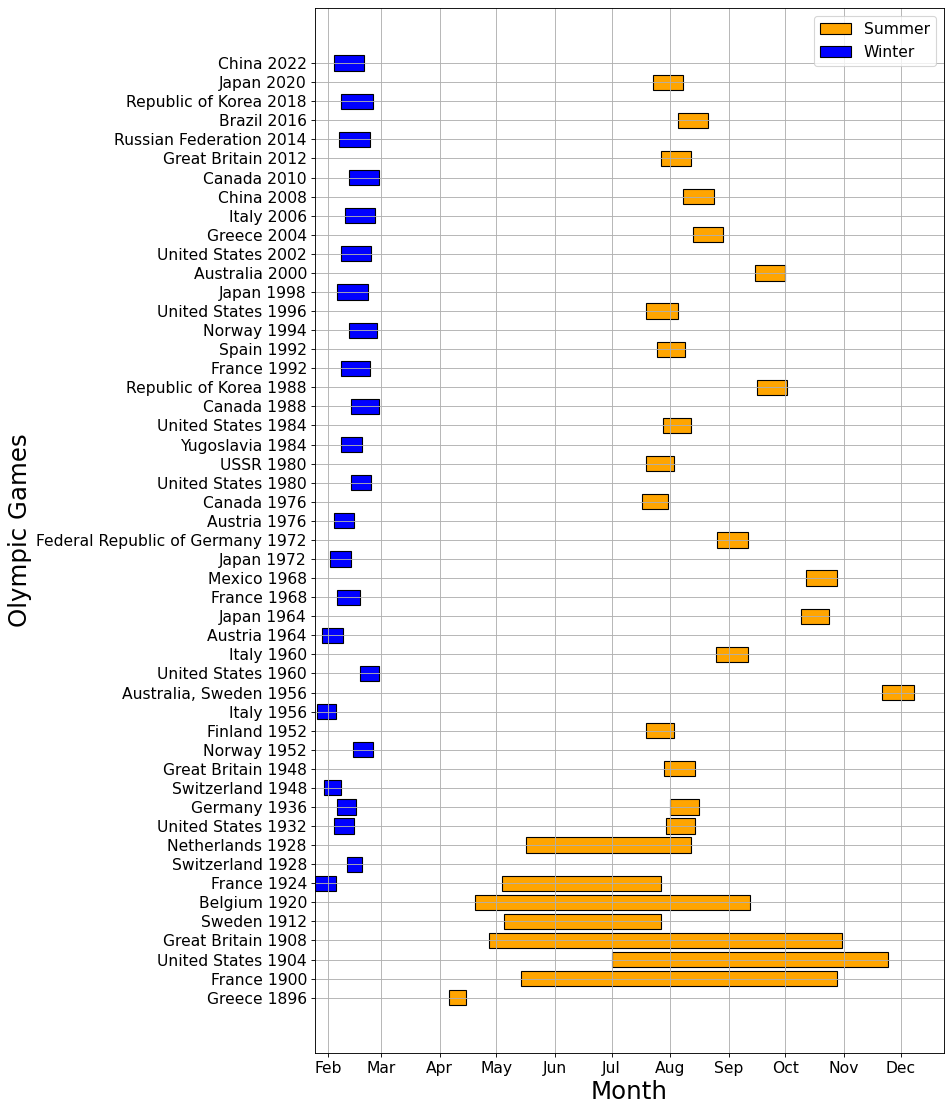
\includegraphics[width=0.8\textwidth]{Gantt Chart of Olympic Games.png}
    \caption{Gantt Chart of Olympic Games Duration}
    \label{fig:gantt_olympics}
\end{figure}

The modern Olympics began in 1896 with exclusively male participants and a limited schedule of events lasting 10 days. By 1900, the Paris Games introduced women's participation and expanded the schedule to over five months, integrating the Olympics into the World’s Fair. This unusual duration reflected the scattered organization and the addition of new sports like golf, tennis, and rowing. Over time, the duration became more standardized, with events typically lasting around two weeks by the mid-20th century, reflecting the Games' growing scale and complexity.

The Winter Olympics were introduced in Chamonix, France, in 1924, marking the start of a separate seasonal competition for winter sports. Notably, France hosted both the Summer and Winter Games in the same year, solidifying its pivotal role in Olympic history.

Additionally, the chart captures regular scheduling patterns, with Summer Games typically held between July and August and Winter Games in February. It also reveals disruptions caused by global conflicts, including cancellations during World War I and World War II.

\section{Chord Diagram for Migration Flow}

Given the increasing rate of immigration over the past few decades, we decided to analyze immigration in the context of the Olympic Games, specifically focusing on Olympic athletes who represent countries different from the ones in which they were born. A key component for this analysis was the inclusion of athletes' birth countries, which were not initially present in the dataset. To address this, we used web scraping to extract athletes' birth countries from their Wikipedia pages and added this information as a new feature to the dataset. Since there have been significant changes in the names and territories of countries over time, we decided to focus only on the last 10 Olympic Games to ensure consistency.

To visualize this analysis, we used a chord diagram. A chord diagram is a graphical tool designed to show relationships between entities, where the flow of migration is represented by the chords. The source and destination countries of the migration are indicated by the base and arrowhead of each chord, respectively. The width of each arc is proportional to the number of athletes migrating from one country to another.

In our chord diagram, the countries are grouped by sub-continent, with a total of 9 sub-continents, plus the Refugee Olympic Team, which is treated as a separate category. Each sub-continent is assigned a unique color theme to improve the clarity of the visualization. To make the analysis more manageable and focused, we only included countries with more than 10 immigrant athletes in the diagram. This filter ensures that the visualization highlights significant migration flows.

\begin{figure}[ht]
    \centering
    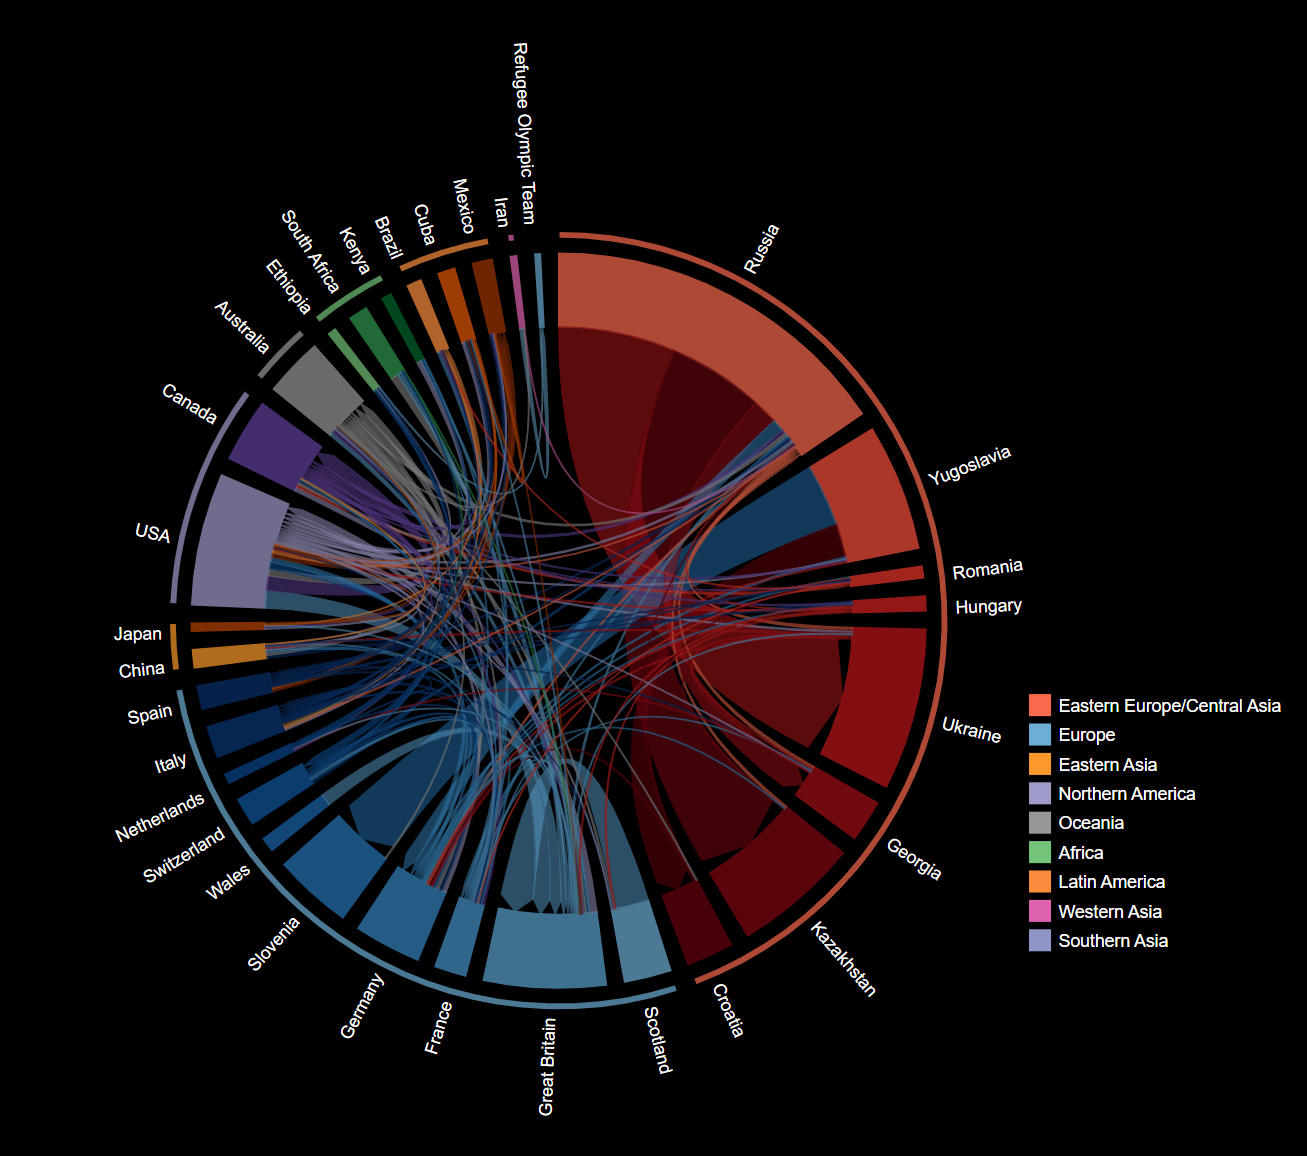
\includegraphics[width=0.8\textwidth]{chord_diagram.png}
    \caption{Chord Diagram: Visualizing Olympic Athletes' Migration Flows Since 2010}
    \label{fig:chord_diagram}
\end{figure}

\subsection{Features of the Diagram}
An interactive feature of this diagram is that when hovering over a country's name, additional information is displayed, including the total number of incoming and outgoing immigrants for that country. Additionally, when hovering over a country, the opacity of arrows that do not originate from or end in that country is reduced. This allows the user to focus on immigration flows specifically related to the selected country, highlighting it as the source or destination
\subsection{Insights from the Diagram}
The diagram provides valuable insights into immigration patterns. Most visible immigration flows align closely with political and geographical changes in the world. In particular, highly developed countries like the United States and Britain emerge as major destinations for immigrants, likely due to the better opportunities and higher quality of life they offer.

However, the diagram also reveals patterns specific to the unique nature of the dataset. For instance, Russia was banned from participating in the 2016 Rio and 2020 Tokyo Olympics due to doping violations. In such cases, many Russian athletes opted to compete under other countries' flags just to continue participating in the games.

Another intriguing trend is the movement of athletes between countries in pursuit of better athletic opportunities. For example, some U.S. athletes appear to have moved to Latin American countries, possibly because it was easier to qualify for the Olympic team there.


\section{Dynamic Choropleths and Bubble Maps}

The dynamic choropleth and bubble maps were designed to provide an interactive exploration of Olympic trends worldwide. These maps enable users to visualize data such as the frequency of Olympic hosting by country, the number of athlete debuts, and medal counts. With dynamic filtering options and multiple visualization styles, they offer a versatile and engaging way to analyze key aspects of Olympic history.

The choropleth map excels at conveying spatial patterns and regional comparisons through color intensity, making it ideal for quickly identifying geographical trends. However, it may obscure information for smaller countries due to their limited map space. In contrast, the bubble map highlights individual data points with proportional circle sizes, ensuring that smaller countries remain visible and providing a more precise representation of numerical values. On the downside, bubble maps can become cluttered in regions with dense data points, potentially making it harder to interpret overlapping bubbles. Together, these visualization styles complement each other, balancing clarity and detail depending on the user's analytical needs.

\begin{figure}[ht]
    \centering
    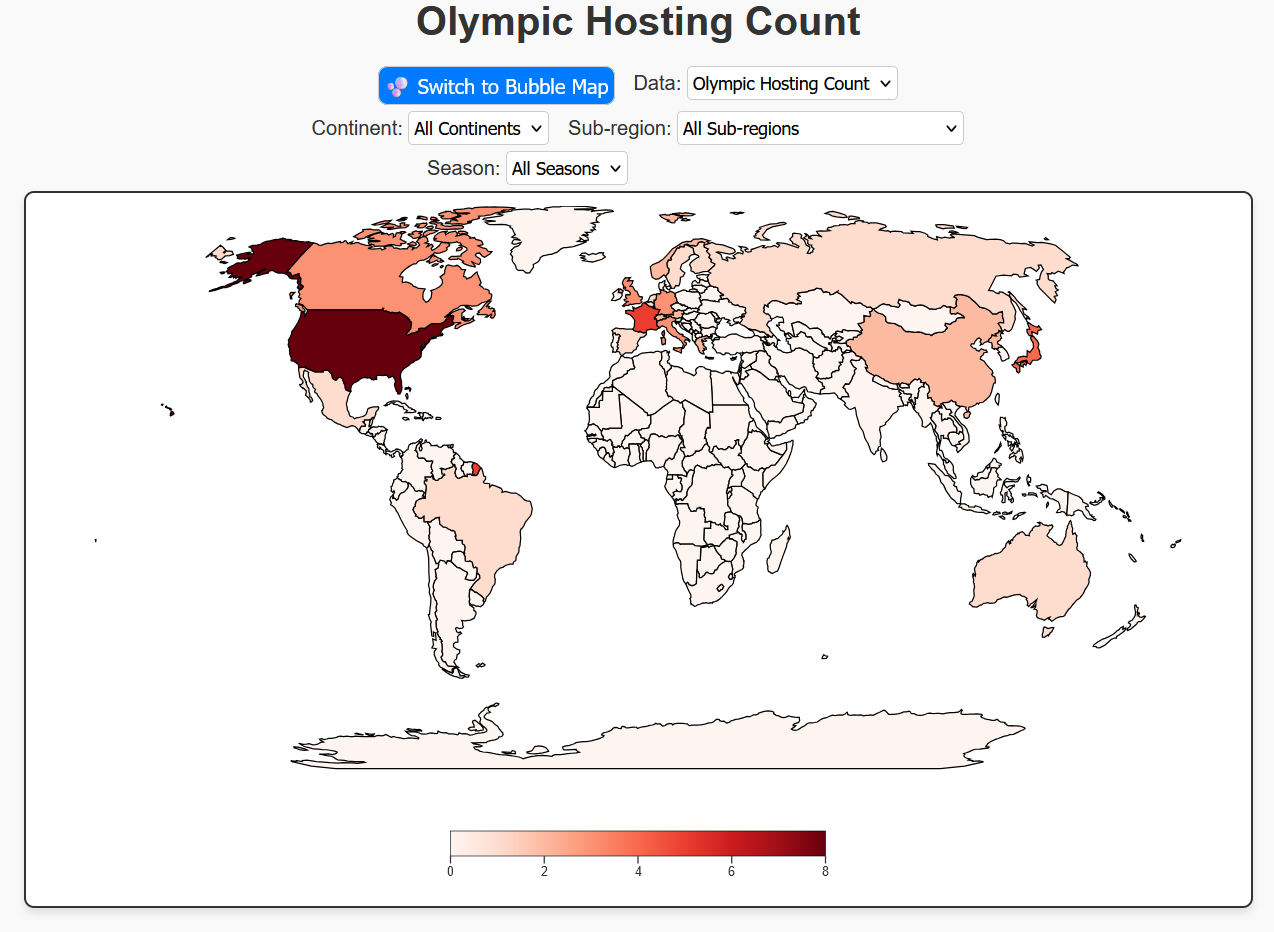
\includegraphics[width=0.8\textwidth]{Dynamic Choropleth.png}
    \caption{Dynamic Choropleth Map: Visualizing Olympic Hosting Trends}
    \label{fig:choropleth_map}
\end{figure}

\begin{figure}[ht]
    \centering
    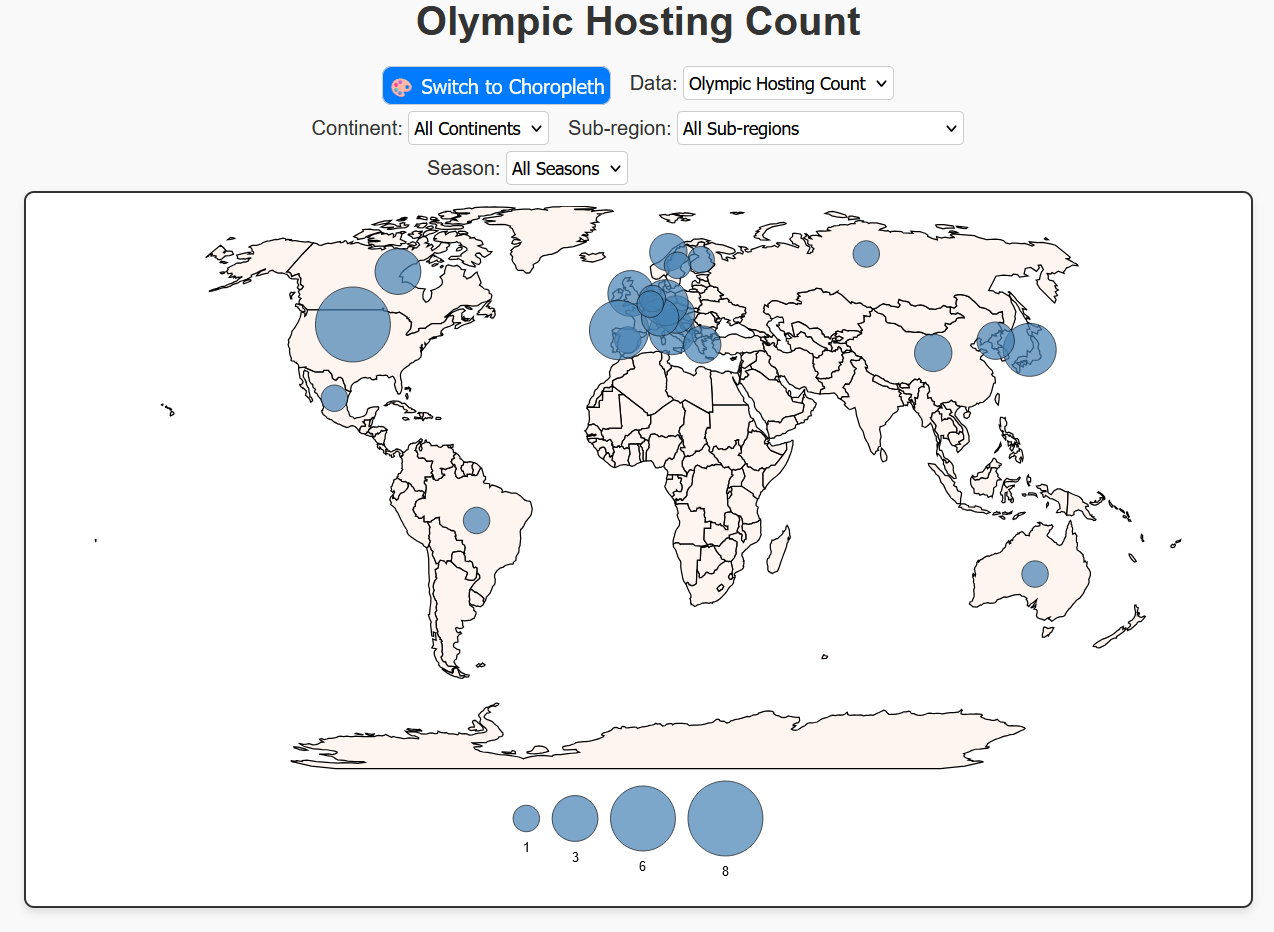
\includegraphics[width=0.8\textwidth]{Dynamic Bubble Map.png}
    \caption{Dynamic Bubble Map: Visualizing Olympic Hosting Trends}
    \label{fig:bubble_map}
\end{figure}

\subsection{Features of the Maps}

The maps provide the following functionalities:
\begin{itemize}
    \item \textbf{Visualization Modes:} Users can switch between a choropleth map (Figure \ref{fig:choropleth_map}) and a bubble map (Figure \ref{fig:bubble_map}) for different visual representations of hosting frequency.
    \item \textbf{Filters and Options:} Filtering options include continents, sub-regions, seasons (Summer or Winter), medal types (Gold, Silver or Bronze), if applicable. These allow users to customize the view and focus on specific geographic or temporal trends.
    \item \textbf{Interactivity:} Both maps feature hover-over tooltips displaying detailed information, such as the number of times a country has hosted the Olympics.
\end{itemize}

\subsection{Insights from the Maps}

These maps reveal several insights into Olympic hosting trends:
\begin{itemize}
    \item Countries such as the United States, Great Britain, and France stand out in number of debuts and high hosting frequencies, reflecting their longstanding involvement in the Olympics.
    \item Hosting occurrences are concentrated in Europe and North America, particularly during the early years of the modern Olympics.
    \item The inclusion of filtering options enables the identification of hosting trends by region, season, and medal type, highlighting the geographical expansion of the Games over time.
\end{itemize}

The combination of choropleth and bubble maps exemplifies the power of interactive visualizations, enabling a flexible exploration of the data while revealing key trends and disparities in Olympic hosting.

\section{Interactive Cumulative Medals Visualization}

This section introduces an interactive visualization that dynamically displays the evolution of cumulative Olympic medals for the top 20 countries, based on total medal counts from 1896 to 2022. The visualization allows users to select specific countries, adjust the animation speed, and explore trends over time.

\begin{figure}[ht]
    \centering
    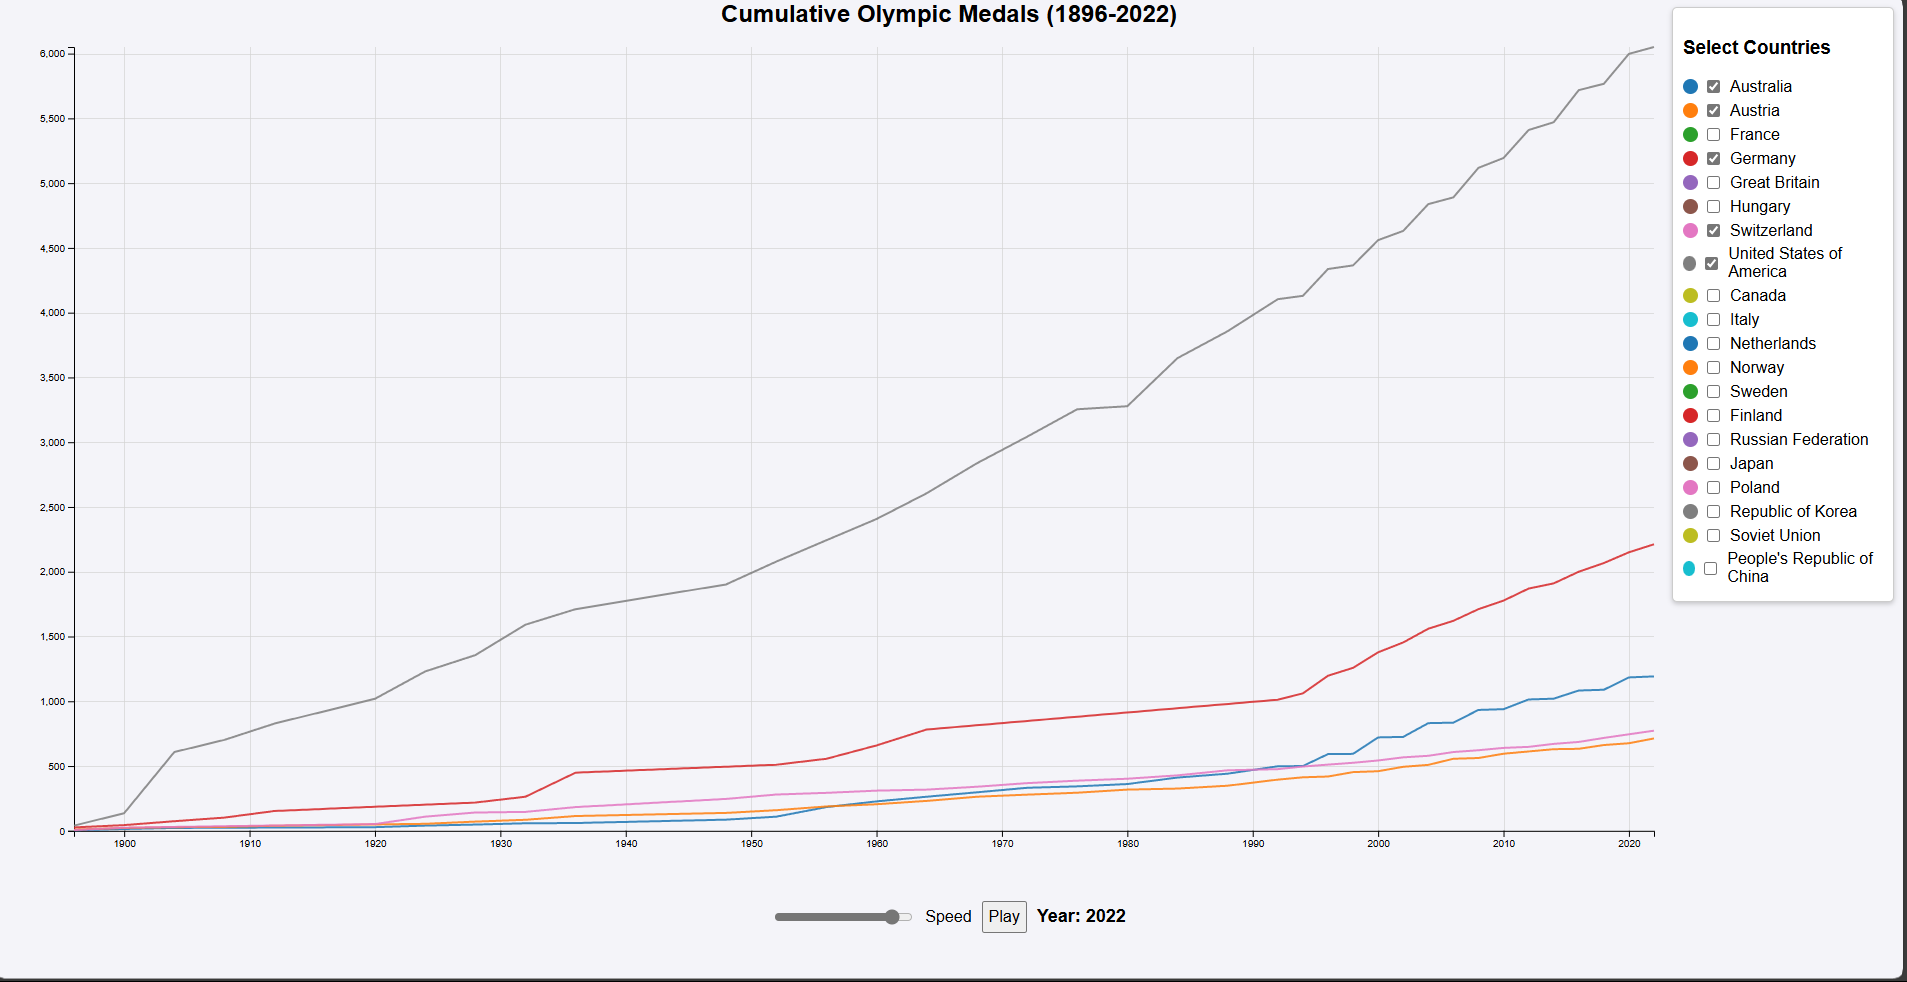
\includegraphics[width=0.8\textwidth]{cumulative_medal_count.png}
    \caption{Interactive Line Chart of Cumulative Olympic Medals}
    \label{fig:line_chart_cumulative_medals}
\end{figure}

\subsection{Features of the Visualization}

The interactive line chart provides the following functionalities:
\begin{itemize}
    \item \textbf{Dynamic Country Selection:} A control panel allows users to select countries of interest, focusing the visualization on specific datasets.
    \item \textbf{Adjustable Speed:} Users can modify the animation speed through a slider, enabling both detailed and high-level explorations.
    \item \textbf{Dynamic Axes and Gridlines:} Axes and gridlines adjust dynamically during the animation, ensuring a clear representation of trends.
    \item \textbf{Year Tracking:} A label dynamically updates to display the current year during the animation, providing a temporal reference.
\end{itemize}

\subsection{Insights from the Visualization}

This visualization offers several insights into Olympic medal trends:
\begin{itemize}
    \item Countries such as the United States, Soviet Union, and Great Britain demonstrate consistently high cumulative medal counts, reflecting their historical dominance in the Olympics.
    \item Newer Olympic nations exhibit rapid growth in cumulative medals, showcasing their emerging success over time.
    \item The interactive nature allows users to identify key turning points, such as the effects of global events (e.g., World Wars) on medal accumulation.
\end{itemize}

This visualization exemplifies the potential of dynamic and interactive tools in enhancing the exploration and understanding of historical data trends.


\section{Olympic Medal Density Visualization}

This section introduces an interactive map visualization of Olympic medal distributions over time. The map, shown in Figure \ref{fig:olympic_medal_density_map}, dynamically displays the density of medals won by countries in each Olympic Games from 1980 to 2022, allowing users to explore geographical trends in medal achievements.

\begin{figure}[ht]
    \centering
    \includegraphics[width=0.8\textwidth]{Olympic_Medal_Density_Map.png}
    \caption{Olympic Medal Density Map: Medal Distributions by Country (1980-2022)}
    \label{fig:olympic_medal_density_map}
\end{figure}

\subsection{Features of the Visualization}

This interactive map includes the following functionalities:
\begin{itemize}
    \item \textbf{Dynamic Medal Visualization:} Countries are shaded based on the total number of medals won, with darker colors indicating higher medal counts.
    \item \textbf{Year Slider:} A slider allows users to select specific years, updating the map to reflect medal distributions for that year.
    \item \textbf{Tooltip Interactivity:} Hovering over a country displays detailed information about its medal achievements, including counts for Gold, Silver, Bronze, and Total medals.
    \item \textbf{Color Legend:} A color bar legend provides a reference for interpreting the shading intensity, corresponding to medal density.
\end{itemize}

\subsection{Insights from the Visualization}

This visualization reveals significant patterns in Olympic medal distributions:
\begin{itemize}
    \item Traditional powerhouses like the United States, Russia, and China consistently dominate the medal tallies, highlighted by darker shades on the map.
    \item Regional trends, such as strong performances by European nations and emerging contributions from African and Asian countries, become apparent over time.
    \item Disruptions in medal patterns during specific years, such as the Cold War-era boycotts of 1980 and 1984, are easily observable.
    \item The interactive slider enables a temporal analysis, allowing users to trace the evolution of Olympic success across decades.
\end{itemize}

This map provides an engaging and intuitive way to explore the geographical distribution of Olympic success, offering insights into historical trends and emerging nations in the Olympic arena.


\section{Olympic Rivalries Network Visualization}

This section presents an interactive network visualization that explores the complex relationships and rivalries between countries in the Olympic Games. The visualization, shown in Figure \ref{fig:olympic_rivalries_network}, highlights countries' total medal counts and their competitive interactions over time, with connections emphasizing shared participation in events.

\begin{figure}[ht]
    \centering
    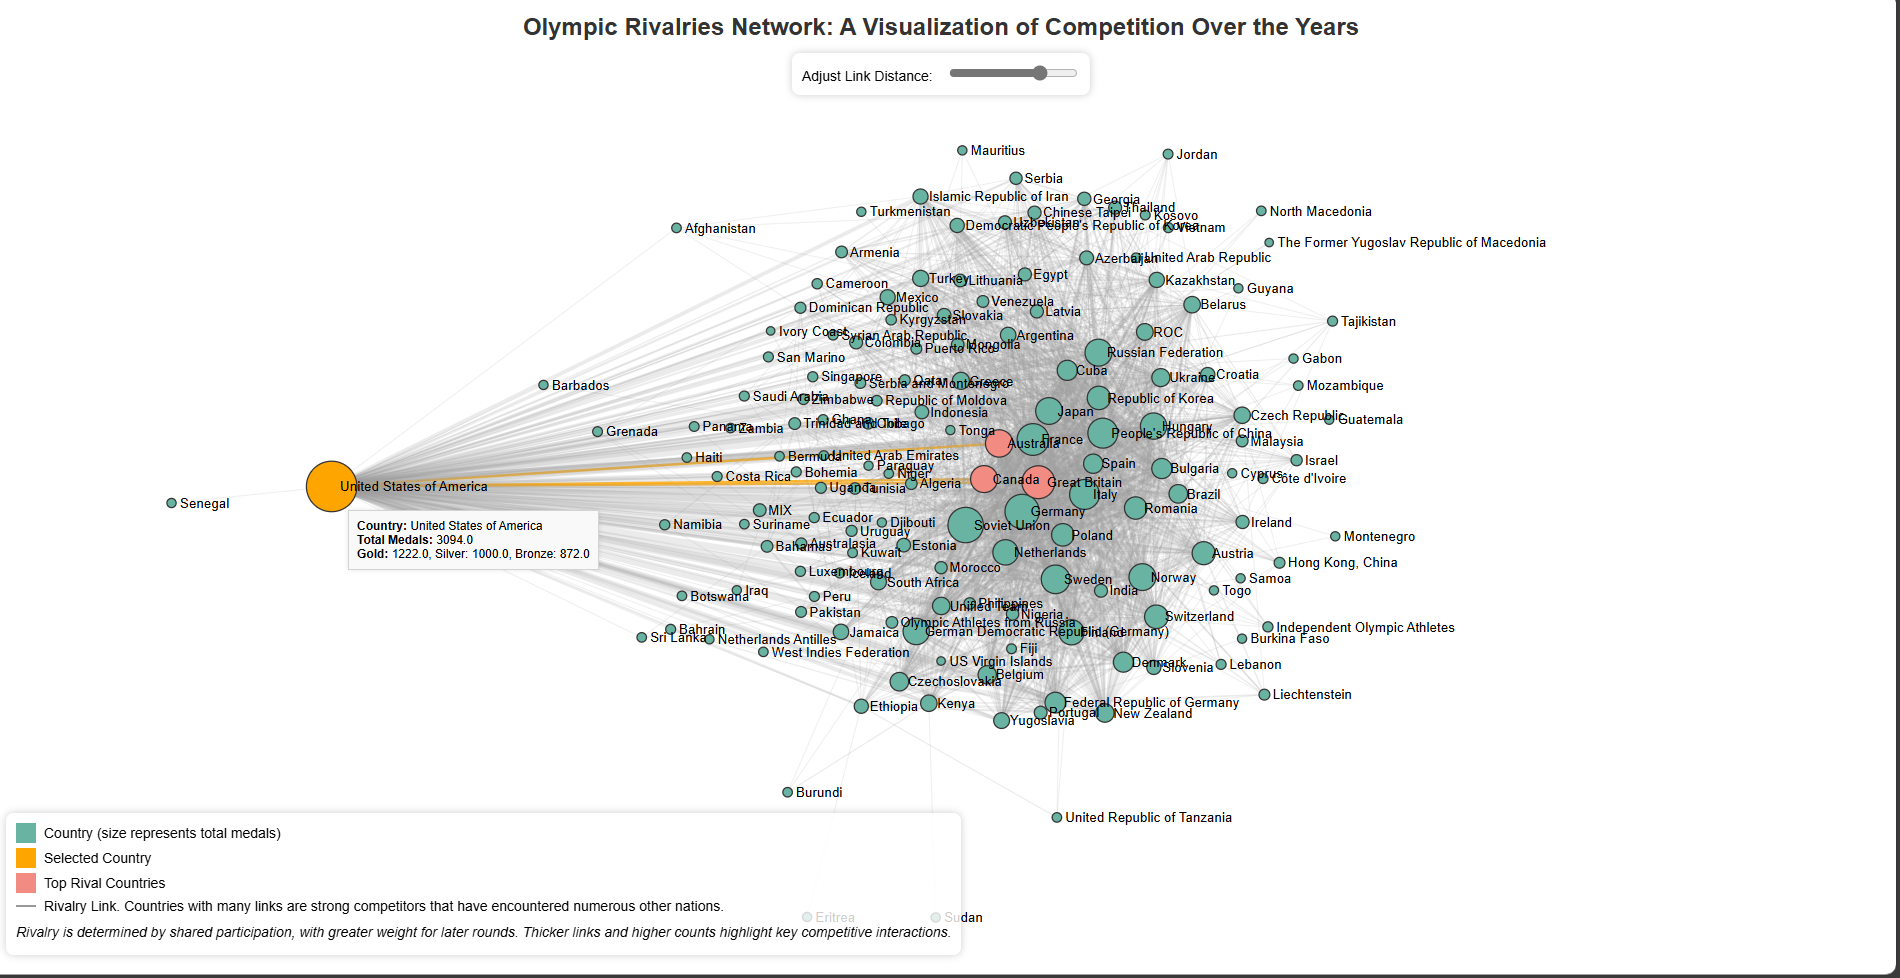
\includegraphics[width=0.8\textwidth]{graph_viz.png}
    \caption{Interactive Olympic Rivalries Network: Countries and Medal Links}
    \label{fig:olympic_rivalries_network}
\end{figure}

\subsection{Features of the Visualization}

The interactive network provides the following functionalities:
\begin{itemize}
    \item \textbf{Node Representation:} Each node represents a country, with its size proportional to the total number of medals won.
    \item \textbf{Link Representation:} Links between nodes represent competitive interactions, with thicker links indicating stronger rivalries based on shared participation, especially in later rounds.
    \item \textbf{Interactivity:}
          \begin{itemize}
              \item Hovering over nodes displays a tooltip with the country name, total medals, and medal breakdown by type (Gold, Silver, Bronze).
              \item Clicking a node highlights the top three rival countries and their competitive links.
          \end{itemize}
    \item \textbf{Dynamic Adjustments:} A slider allows users to adjust the link distance, dynamically reorganizing the network for clarity.
    \item \textbf{Legend:} A detailed legend explains the meaning of node sizes, colors, and link thickness, ensuring user accessibility and understanding.
\end{itemize}

\subsection{Insights from the Visualization}

The Olympic Rivalries Network provides unique insights into the relationships and rivalries between countries:
\begin{itemize}
    \item Countries with higher medal counts, such as the United States, Russia, and China, emerge as central nodes with numerous connections, highlighting their dominance in the Olympics.
    \item Strong rivalries are evident between geographically or politically significant nations, such as the USA and USSR during the Cold War era.
    \item Smaller nations with significant connections, such as Jamaica in athletics or Kenya in long-distance running, showcase specialized rivalries in specific sports.
    \item The interactive design allows users to explore the evolving competitive dynamics over time, emphasizing the global nature of the Olympics.
\end{itemize}

This visualization exemplifies the power of network analysis in uncovering patterns and relationships in complex datasets, offering a dynamic and engaging perspective on Olympic history.

\section{Analysis of Olympic Participation Trends Over Time}

This section provides an analysis of the trends in global participation in the Olympic Games from their inception in 1896 to the most recent Games in 2021. The visualization in Figure \ref{fig:olympic_participation_trends} captures the number of countries participating in each Olympic Games, highlighting key historical events and their impact on participation.

\begin{figure}[ht]
    \centering
    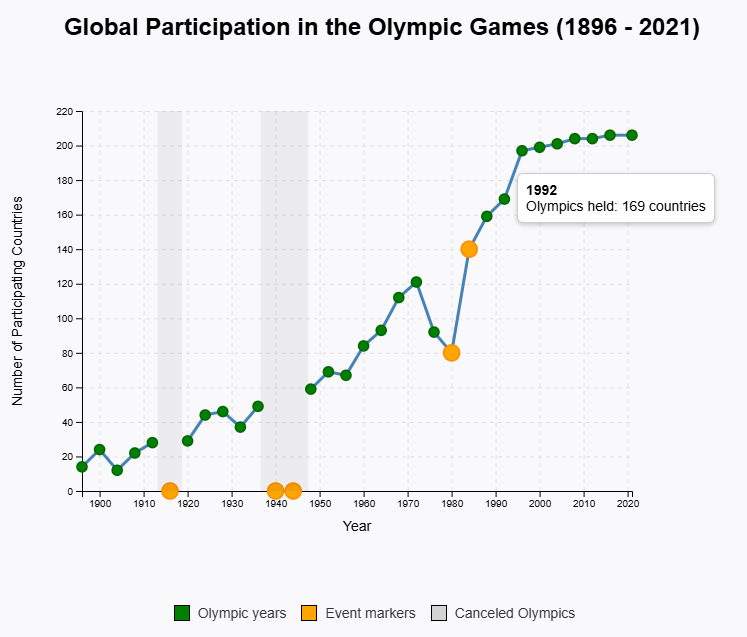
\includegraphics[width=0.8\textwidth]{participation_in_olympics.png}
    \caption{Olympic Participation Trends: Number of Participating Countries (1896-2021)}
    \label{fig:olympic_participation_trends}
\end{figure}

\subsection{Features of the Visualization}

This interactive line chart and marker-based visualization include the following elements:
\begin{itemize}
    \item \textbf{Participation Trends:} A blue line representing the number of countries participating in each Olympic Games, excluding canceled years.
    \item \textbf{Event Markers:} Circles highlighting key historical events, such as World War-related cancellations and notable boycotts.
    \item \textbf{Shaded Regions:} Gray regions marking periods when the Olympics were canceled (e.g., during World War I and World War II).
    \item \textbf{Interactive Tooltips:} Hovering over points provides detailed information about the year, number of participating countries, and significant events.
    \item \textbf{Legend:} A color-coded legend explains the meaning of the different visual elements, ensuring clarity and accessibility.
\end{itemize}

\subsection{Insights from the Visualization}

This visualization reveals several key insights into Olympic participation trends:
\begin{itemize}
    \item Participation steadily increased from 14 countries in the inaugural Games to 206 countries in recent editions, reflecting the Olympics' growing global appeal.
    \item Significant dips in participation occurred during the 1980 and 1984 Games due to Cold War-era boycotts.
    \item Periods of cancellations during World War I and World War II (1916, 1940, and 1944) are clearly marked, emphasizing the impact of global conflicts on the Olympics.
    \item The introduction of new nations in the post-World War II era led to a sharp rise in participation, with notable milestones in the 1992 Games (169 countries) and the post-Cold War 1996 Games (197 countries).
\end{itemize}

By combining historical context with interactive elements, this visualization provides a comprehensive overview of how global events and geopolitical shifts have shaped the Olympic Games over time.

\section{Data Dashboard}

This HTML page serves as a centralized hub for all visualizations, consolidating plots and charts to offer a clear and organized view of the data. Each plot acts as a clickable link, redirecting users to the corresponding full visualization page. A description overlay appears on hover, providing additional context for each plot.

The page leverages various HTML and CSS features, including iframe for embedding visualizations, zoom and transform for dynamic scaling, and hover effects for interactivity. Additionally, the responsive grid layout ensures the visualizations adapt seamlessly to different screen sizes, maintaining proper spacing and alignment for an optimized user experience.

\begin{figure}[ht]
    \centering
    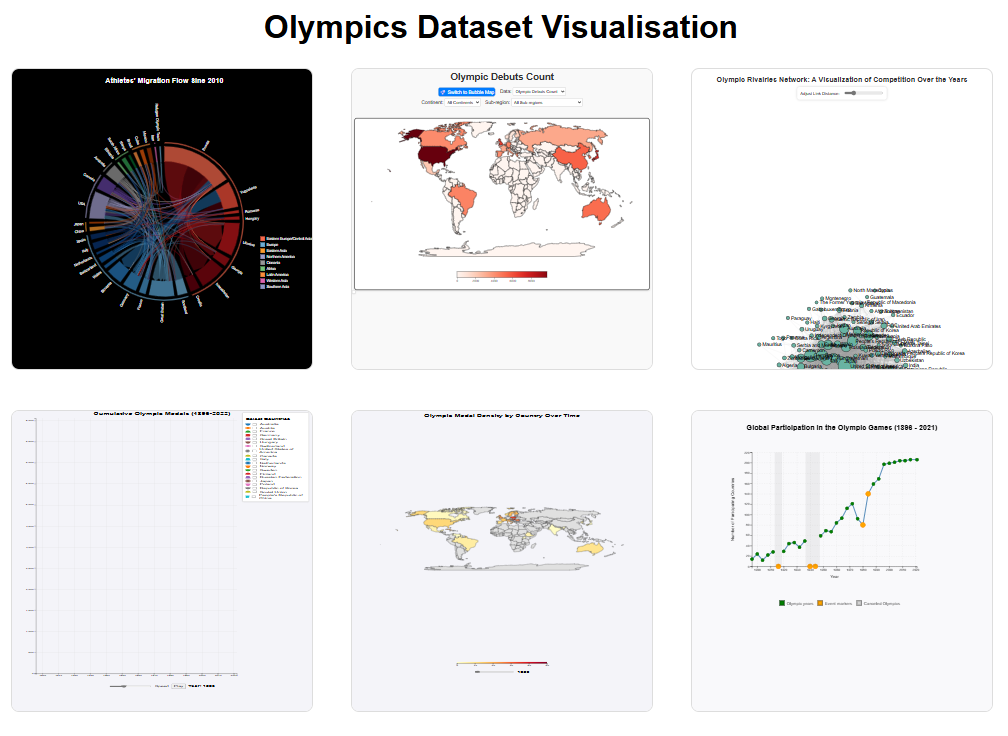
\includegraphics[width=0.8\textwidth]{DataDashboard.png}
    \caption{Data Dashboard: A centralized hub for displaying and accessing all visualizations}
    \label{fig:dashboard}
\end{figure}
